% ===============================================================
% Entrega 5: Prototipo Funcional Completo do Bloom em Vulkan
% Incluido no main.tex com % ===============================================================
% Entrega 5: Prototipo Funcional Completo do Bloom em Vulkan
% Incluido no main.tex com % ===============================================================
% Entrega 5: Prototipo Funcional Completo do Bloom em Vulkan
% Incluido no main.tex com % ===============================================================
% Entrega 5: Prototipo Funcional Completo do Bloom em Vulkan
% Incluido no main.tex com \input{entrega5}
% ===============================================================

\section{Protótipo Funcional Completo em Vulkan}
\label{sec:prototipo}
\sloppy

Esta seção documenta a entrega do protótipo funcional completo da técnica de \textit{Bloom} e pós-processamento em tempo real. O código desenvolvido integra a arquitetura de 11 passes e 5 \textit{render passes} projetada na Entrega 2 (Seção~\ref{sec:arquitetura}) aos \textit{shaders} em GLSL compilados para SPIR-V da Entrega 3 (Seção~\ref{sec:pseudocodigo}), executando sobre o \textit{boilerplate} construído na Entrega 4 (Seção~\ref{sec:boilerplate}).

\subsection{Arquitetura e Fluxo de Execução na GPU}
O protótipo executa o ciclo completo de pós-processamento gráfico em tempo real para cada quadro apresentado:

\begin{enumerate}
    \setlength{\itemsep}{0pt}
    \item \textbf{Passe 0 (Cena 3D HDR):} Renderiza um modelo tridimensional rotativo com iluminação difusa Lambertiana e áreas de emissão de alta intensidade (\textit{neon}). A saída é gravada em ponto flutuante de 16 bits na imagem \texttt{sceneHDR} (\texttt{VK\_FORMAT\_R16G16B16A16\_SFLOAT}) com suporte a teste de profundidade via \texttt{depthImage}.
    \item \textbf{Barreira B1:} Transiciona a imagem \texttt{sceneHDR} do layout \texttt{COLOR\_ATTACHMENT\_OPTIMAL} para \texttt{SHADER\_READ\_ONLY\_OPTIMAL}.
    \item \textbf{Passe 1 (Bright Pass):} Executa o \texttt{bright.frag} sobre o triângulo de tela cheia, avaliando a luminância de cada bloco $2\times2$ e aplicando o corte suave (\textit{soft knee}, Equação~\ref{eq:softknee}) para isolar fragmentos com luminância superior a $1.0$, escrevendo em \texttt{bloomMip[0]} com metade da resolução nativa.
    \item \textbf{Barreira B2:} Transiciona \texttt{bloomMip[0]} para leitura como textura.
    \item \textbf{Passes 2 a 5 (Downsample Piramidal):} Encadeia 4 execuções do \texttt{downsample.frag} utilizando o filtro de 13 amostras (Equação~\ref{eq:gauss}), gerando progressivamente os níveis \texttt{bloomMip[1]} a \texttt{bloomMip[4]} com resoluções decrescentes e aplicando as respectivas barreiras de sincronização B3 a B6.
    \item \textbf{Passes 6 a 9 (Upsample Piramidal com Mistura Aditiva):} Encadeia 4 execuções do \texttt{upsample.frag} com o filtro tenda $3\times3$, interpolando os níveis menores e acumulando os dados nos níveis maiores via \textit{Additive Blending} (\texttt{VK\_BLEND\_FACTOR\_ONE} na origem e no destino) com as barreiras B7 a B10. Ao término do Passe 9, o nível \texttt{bloomMip[0]} armazena o halo de dispersão volumétrica completo.
    \item \textbf{Passe 10 (Composição e Tone Mapping):} Executa o \texttt{composite.frag}, combinando aditivamente a cena original \texttt{sceneHDR} com o halo de \textit{Bloom} ponderado pelo fator de intensidade $\alpha$, aplicando o mapeamento tonal de Reinhard (Equação~\ref{eq:reinhard}) e gravando o resultado final na imagem da \textit{swapchain} para apresentação ao monitor.
\end{enumerate}

\subsection{Comprovação Visual e Análise Comparativa}
Para comprovar cientificamente o funcionamento da técnica, o protótipo inclui um mecanismo de controle dinâmico que permite ligar e desligar o \textit{Bloom} em tempo real. A Figura~\ref{fig:comparativo_bloom} apresenta a comparação direta capturada da memória da GPU.

\begin{figure}[H]
    \centering
    \begin{minipage}{0.48\textwidth}
        \centering
        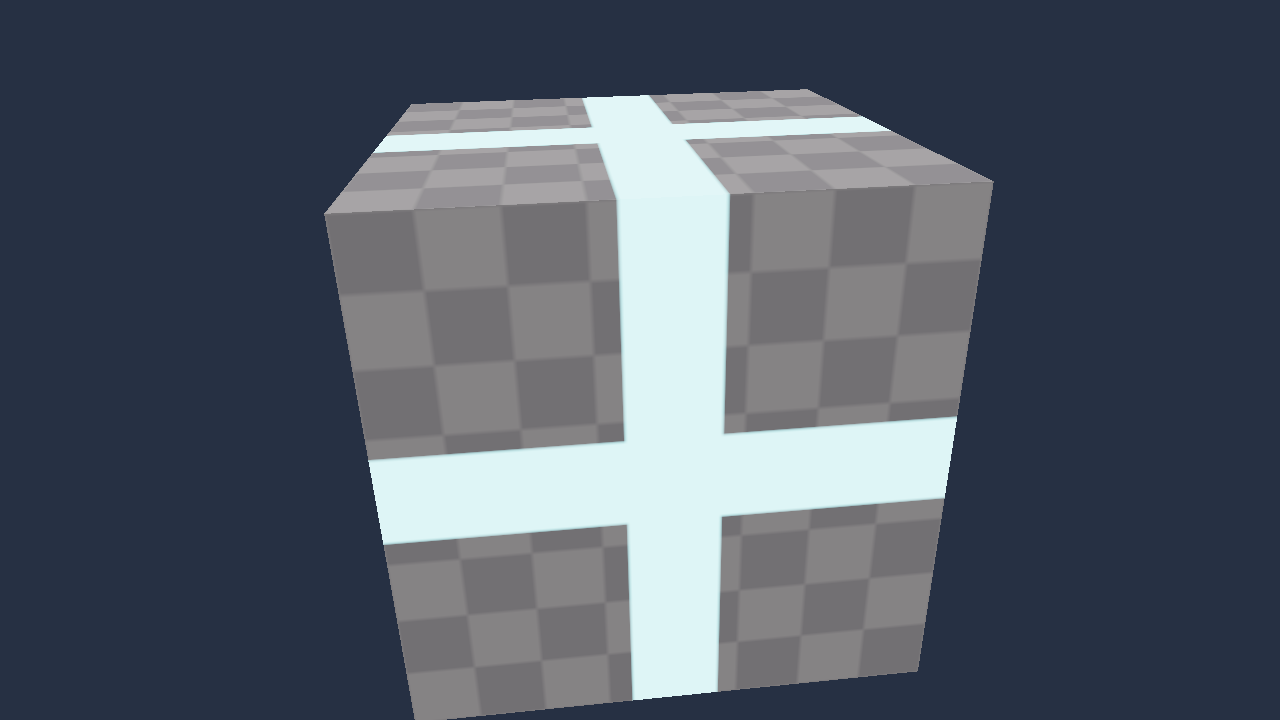
\includegraphics[width=\linewidth]{captura_bloom_desativado.png}
        \textbf{(a) Sem Bloom (LDR puro)}
    \end{minipage}
    \hfill
    \begin{minipage}{0.48\textwidth}
        \centering
        
\includegraphics[width=\linewidth]{captura_bloom_ativo.png}
        \textbf{(b) Com Bloom Ativo}
    \end{minipage}
    \caption{Comparação direta gerada pelo protótipo Vulkan. Em (a), a faixa incandescente sofre corte abrupto sem simulação de dispersão; em (b), o pipeline completo de 11 passes produz o espalhamento suave da luz (\textit{light bleeding}) ao redor do objeto, conferindo a percepção física de extrema luminância.}
    \label{fig:comparativo_bloom}
\end{figure}

\subsection{Interatividade e Usabilidade do Protótipo}
O protótipo permite intervenção direta do usuário em tempo de execução através das seguintes teclas:
\begin{itemize}
    \setlength{\itemsep}{0pt}
    \item \textbf{Barra de Espaço:} Alterna instantaneamente entre o modo com \textit{Bloom} ativo e o modo desativado, viabilizando a demonstração comparativa ao vivo.
    \item \textbf{Teclas \texttt{+} e \texttt{-}:} Aumentam e diminuem a intensidade do espalhamento luminoso ($\alpha$).
    \item \textbf{Tecla \texttt{ESC}:} Encerra a aplicação de forma limpa, garantindo a destruição ordenada de todos os semáforos, \textit{fences}, imagens e \textit{buffers} alocados na GPU.
\end{itemize}
\fussy

% ===============================================================

\section{Protótipo Funcional Completo em Vulkan}
\label{sec:prototipo}
\sloppy

Esta seção documenta a entrega do protótipo funcional completo da técnica de \textit{Bloom} e pós-processamento em tempo real. O código desenvolvido integra a arquitetura de 11 passes e 5 \textit{render passes} projetada na Entrega 2 (Seção~\ref{sec:arquitetura}) aos \textit{shaders} em GLSL compilados para SPIR-V da Entrega 3 (Seção~\ref{sec:pseudocodigo}), executando sobre o \textit{boilerplate} construído na Entrega 4 (Seção~\ref{sec:boilerplate}).

\subsection{Arquitetura e Fluxo de Execução na GPU}
O protótipo executa o ciclo completo de pós-processamento gráfico em tempo real para cada quadro apresentado:

\begin{enumerate}
    \setlength{\itemsep}{0pt}
    \item \textbf{Passe 0 (Cena 3D HDR):} Renderiza um modelo tridimensional rotativo com iluminação difusa Lambertiana e áreas de emissão de alta intensidade (\textit{neon}). A saída é gravada em ponto flutuante de 16 bits na imagem \texttt{sceneHDR} (\texttt{VK\_FORMAT\_R16G16B16A16\_SFLOAT}) com suporte a teste de profundidade via \texttt{depthImage}.
    \item \textbf{Barreira B1:} Transiciona a imagem \texttt{sceneHDR} do layout \texttt{COLOR\_ATTACHMENT\_OPTIMAL} para \texttt{SHADER\_READ\_ONLY\_OPTIMAL}.
    \item \textbf{Passe 1 (Bright Pass):} Executa o \texttt{bright.frag} sobre o triângulo de tela cheia, avaliando a luminância de cada bloco $2\times2$ e aplicando o corte suave (\textit{soft knee}, Equação~\ref{eq:softknee}) para isolar fragmentos com luminância superior a $1.0$, escrevendo em \texttt{bloomMip[0]} com metade da resolução nativa.
    \item \textbf{Barreira B2:} Transiciona \texttt{bloomMip[0]} para leitura como textura.
    \item \textbf{Passes 2 a 5 (Downsample Piramidal):} Encadeia 4 execuções do \texttt{downsample.frag} utilizando o filtro de 13 amostras (Equação~\ref{eq:gauss}), gerando progressivamente os níveis \texttt{bloomMip[1]} a \texttt{bloomMip[4]} com resoluções decrescentes e aplicando as respectivas barreiras de sincronização B3 a B6.
    \item \textbf{Passes 6 a 9 (Upsample Piramidal com Mistura Aditiva):} Encadeia 4 execuções do \texttt{upsample.frag} com o filtro tenda $3\times3$, interpolando os níveis menores e acumulando os dados nos níveis maiores via \textit{Additive Blending} (\texttt{VK\_BLEND\_FACTOR\_ONE} na origem e no destino) com as barreiras B7 a B10. Ao término do Passe 9, o nível \texttt{bloomMip[0]} armazena o halo de dispersão volumétrica completo.
    \item \textbf{Passe 10 (Composição e Tone Mapping):} Executa o \texttt{composite.frag}, combinando aditivamente a cena original \texttt{sceneHDR} com o halo de \textit{Bloom} ponderado pelo fator de intensidade $\alpha$, aplicando o mapeamento tonal de Reinhard (Equação~\ref{eq:reinhard}) e gravando o resultado final na imagem da \textit{swapchain} para apresentação ao monitor.
\end{enumerate}

\subsection{Comprovação Visual e Análise Comparativa}
Para comprovar cientificamente o funcionamento da técnica, o protótipo inclui um mecanismo de controle dinâmico que permite ligar e desligar o \textit{Bloom} em tempo real. A Figura~\ref{fig:comparativo_bloom} apresenta a comparação direta capturada da memória da GPU.

\begin{figure}[H]
    \centering
    \begin{minipage}{0.48\textwidth}
        \centering
        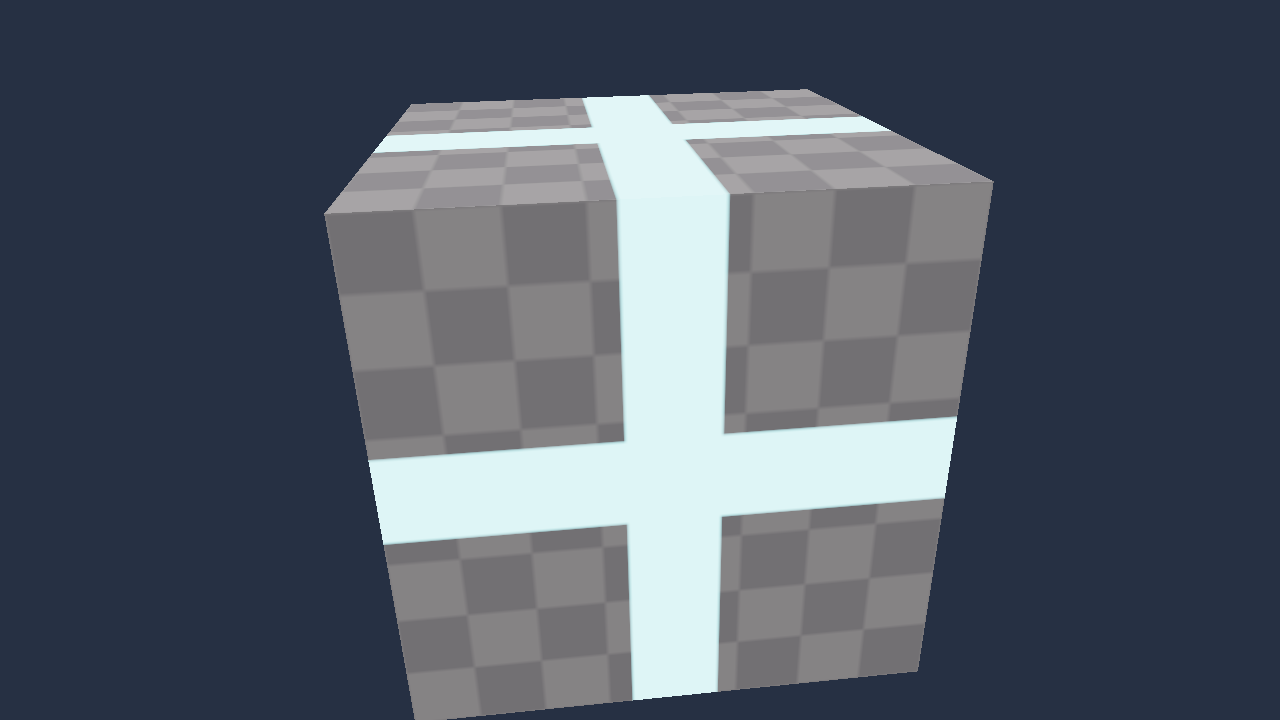
\includegraphics[width=\linewidth]{captura_bloom_desativado.png}
        \textbf{(a) Sem Bloom (LDR puro)}
    \end{minipage}
    \hfill
    \begin{minipage}{0.48\textwidth}
        \centering
        
\includegraphics[width=\linewidth]{captura_bloom_ativo.png}
        \textbf{(b) Com Bloom Ativo}
    \end{minipage}
    \caption{Comparação direta gerada pelo protótipo Vulkan. Em (a), a faixa incandescente sofre corte abrupto sem simulação de dispersão; em (b), o pipeline completo de 11 passes produz o espalhamento suave da luz (\textit{light bleeding}) ao redor do objeto, conferindo a percepção física de extrema luminância.}
    \label{fig:comparativo_bloom}
\end{figure}

\subsection{Interatividade e Usabilidade do Protótipo}
O protótipo permite intervenção direta do usuário em tempo de execução através das seguintes teclas:
\begin{itemize}
    \setlength{\itemsep}{0pt}
    \item \textbf{Barra de Espaço:} Alterna instantaneamente entre o modo com \textit{Bloom} ativo e o modo desativado, viabilizando a demonstração comparativa ao vivo.
    \item \textbf{Teclas \texttt{+} e \texttt{-}:} Aumentam e diminuem a intensidade do espalhamento luminoso ($\alpha$).
    \item \textbf{Tecla \texttt{ESC}:} Encerra a aplicação de forma limpa, garantindo a destruição ordenada de todos os semáforos, \textit{fences}, imagens e \textit{buffers} alocados na GPU.
\end{itemize}
\fussy

% ===============================================================

\section{Protótipo Funcional Completo em Vulkan}
\label{sec:prototipo}
\sloppy

Esta seção documenta a entrega do protótipo funcional completo da técnica de \textit{Bloom} e pós-processamento em tempo real. O código desenvolvido integra a arquitetura de 11 passes e 5 \textit{render passes} projetada na Entrega 2 (Seção~\ref{sec:arquitetura}) aos \textit{shaders} em GLSL compilados para SPIR-V da Entrega 3 (Seção~\ref{sec:pseudocodigo}), executando sobre o \textit{boilerplate} construído na Entrega 4 (Seção~\ref{sec:boilerplate}).

\subsection{Arquitetura e Fluxo de Execução na GPU}
O protótipo executa o ciclo completo de pós-processamento gráfico em tempo real para cada quadro apresentado:

\begin{enumerate}
    \setlength{\itemsep}{0pt}
    \item \textbf{Passe 0 (Cena 3D HDR):} Renderiza um modelo tridimensional rotativo com iluminação difusa Lambertiana e áreas de emissão de alta intensidade (\textit{neon}). A saída é gravada em ponto flutuante de 16 bits na imagem \texttt{sceneHDR} (\texttt{VK\_FORMAT\_R16G16B16A16\_SFLOAT}) com suporte a teste de profundidade via \texttt{depthImage}.
    \item \textbf{Barreira B1:} Transiciona a imagem \texttt{sceneHDR} do layout \texttt{COLOR\_ATTACHMENT\_OPTIMAL} para \texttt{SHADER\_READ\_ONLY\_OPTIMAL}.
    \item \textbf{Passe 1 (Bright Pass):} Executa o \texttt{bright.frag} sobre o triângulo de tela cheia, avaliando a luminância de cada bloco $2\times2$ e aplicando o corte suave (\textit{soft knee}, Equação~\ref{eq:softknee}) para isolar fragmentos com luminância superior a $1.0$, escrevendo em \texttt{bloomMip[0]} com metade da resolução nativa.
    \item \textbf{Barreira B2:} Transiciona \texttt{bloomMip[0]} para leitura como textura.
    \item \textbf{Passes 2 a 5 (Downsample Piramidal):} Encadeia 4 execuções do \texttt{downsample.frag} utilizando o filtro de 13 amostras (Equação~\ref{eq:gauss}), gerando progressivamente os níveis \texttt{bloomMip[1]} a \texttt{bloomMip[4]} com resoluções decrescentes e aplicando as respectivas barreiras de sincronização B3 a B6.
    \item \textbf{Passes 6 a 9 (Upsample Piramidal com Mistura Aditiva):} Encadeia 4 execuções do \texttt{upsample.frag} com o filtro tenda $3\times3$, interpolando os níveis menores e acumulando os dados nos níveis maiores via \textit{Additive Blending} (\texttt{VK\_BLEND\_FACTOR\_ONE} na origem e no destino) com as barreiras B7 a B10. Ao término do Passe 9, o nível \texttt{bloomMip[0]} armazena o halo de dispersão volumétrica completo.
    \item \textbf{Passe 10 (Composição e Tone Mapping):} Executa o \texttt{composite.frag}, combinando aditivamente a cena original \texttt{sceneHDR} com o halo de \textit{Bloom} ponderado pelo fator de intensidade $\alpha$, aplicando o mapeamento tonal de Reinhard (Equação~\ref{eq:reinhard}) e gravando o resultado final na imagem da \textit{swapchain} para apresentação ao monitor.
\end{enumerate}

\subsection{Comprovação Visual e Análise Comparativa}
Para comprovar cientificamente o funcionamento da técnica, o protótipo inclui um mecanismo de controle dinâmico que permite ligar e desligar o \textit{Bloom} em tempo real. A Figura~\ref{fig:comparativo_bloom} apresenta a comparação direta capturada da memória da GPU.

\begin{figure}[H]
    \centering
    \begin{minipage}{0.48\textwidth}
        \centering
        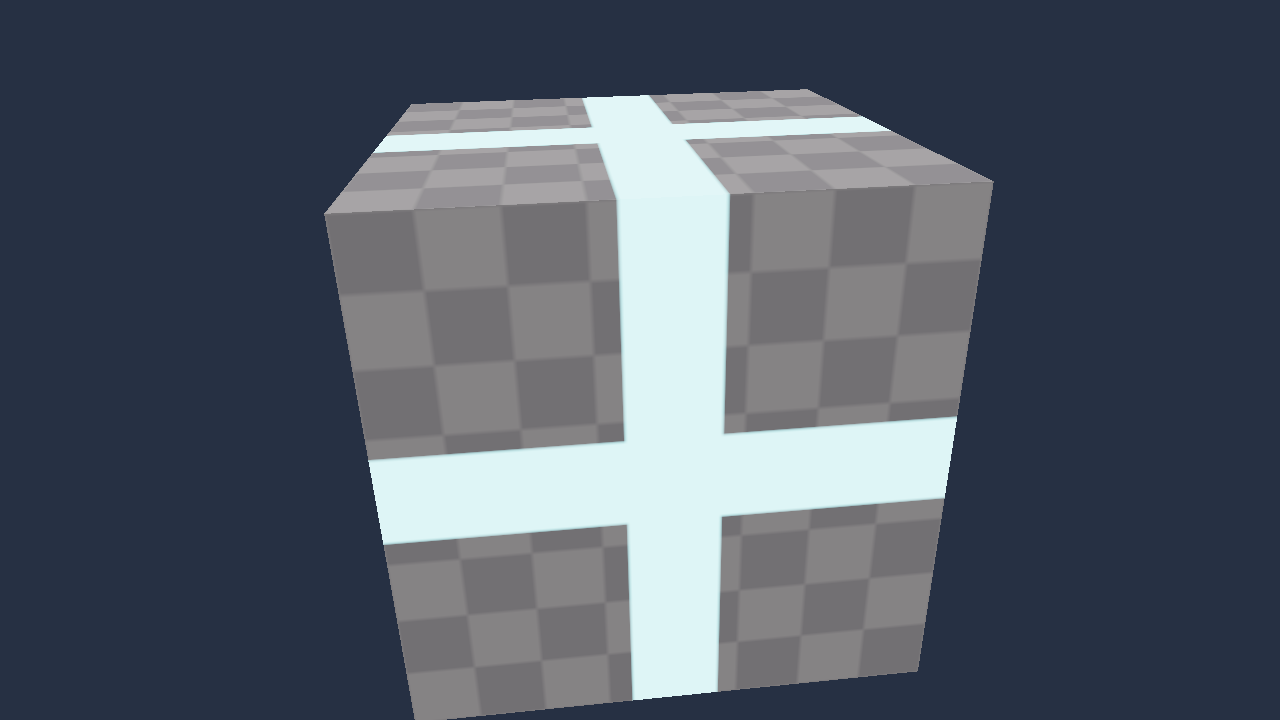
\includegraphics[width=\linewidth]{captura_bloom_desativado.png}
        \textbf{(a) Sem Bloom (LDR puro)}
    \end{minipage}
    \hfill
    \begin{minipage}{0.48\textwidth}
        \centering
        
\includegraphics[width=\linewidth]{captura_bloom_ativo.png}
        \textbf{(b) Com Bloom Ativo}
    \end{minipage}
    \caption{Comparação direta gerada pelo protótipo Vulkan. Em (a), a faixa incandescente sofre corte abrupto sem simulação de dispersão; em (b), o pipeline completo de 11 passes produz o espalhamento suave da luz (\textit{light bleeding}) ao redor do objeto, conferindo a percepção física de extrema luminância.}
    \label{fig:comparativo_bloom}
\end{figure}

\subsection{Interatividade e Usabilidade do Protótipo}
O protótipo permite intervenção direta do usuário em tempo de execução através das seguintes teclas:
\begin{itemize}
    \setlength{\itemsep}{0pt}
    \item \textbf{Barra de Espaço:} Alterna instantaneamente entre o modo com \textit{Bloom} ativo e o modo desativado, viabilizando a demonstração comparativa ao vivo.
    \item \textbf{Teclas \texttt{+} e \texttt{-}:} Aumentam e diminuem a intensidade do espalhamento luminoso ($\alpha$).
    \item \textbf{Tecla \texttt{ESC}:} Encerra a aplicação de forma limpa, garantindo a destruição ordenada de todos os semáforos, \textit{fences}, imagens e \textit{buffers} alocados na GPU.
\end{itemize}
\fussy

% ===============================================================

\section{Protótipo Funcional Completo em Vulkan}
\label{sec:prototipo}
\sloppy

Esta seção documenta a entrega do protótipo funcional completo da técnica de \textit{Bloom} e pós-processamento em tempo real. O código desenvolvido integra a arquitetura de 11 passes e 5 \textit{render passes} projetada na Entrega 2 (Seção~\ref{sec:arquitetura}) aos \textit{shaders} em GLSL compilados para SPIR-V da Entrega 3 (Seção~\ref{sec:pseudocodigo}), executando sobre o \textit{boilerplate} construído na Entrega 4 (Seção~\ref{sec:boilerplate}).

\subsection{Arquitetura e Fluxo de Execução na GPU}
O protótipo executa o ciclo completo de pós-processamento gráfico em tempo real para cada quadro apresentado:

\begin{enumerate}
    \setlength{\itemsep}{0pt}
    \item \textbf{Passe 0 (Cena 3D HDR):} Renderiza um modelo tridimensional rotativo com iluminação difusa Lambertiana e áreas de emissão de alta intensidade (\textit{neon}). A saída é gravada em ponto flutuante de 16 bits na imagem \texttt{sceneHDR} (\texttt{VK\_FORMAT\_R16G16B16A16\_SFLOAT}) com suporte a teste de profundidade via \texttt{depthImage}.
    \item \textbf{Barreira B1:} Transiciona a imagem \texttt{sceneHDR} do layout \texttt{COLOR\_ATTACHMENT\_OPTIMAL} para \texttt{SHADER\_READ\_ONLY\_OPTIMAL}.
    \item \textbf{Passe 1 (Bright Pass):} Executa o \texttt{bright.frag} sobre o triângulo de tela cheia, avaliando a luminância de cada bloco $2\times2$ e aplicando o corte suave (\textit{soft knee}, Equação~\ref{eq:softknee}) para isolar fragmentos com luminância superior a $1.0$, escrevendo em \texttt{bloomMip[0]} com metade da resolução nativa.
    \item \textbf{Barreira B2:} Transiciona \texttt{bloomMip[0]} para leitura como textura.
    \item \textbf{Passes 2 a 5 (Downsample Piramidal):} Encadeia 4 execuções do \texttt{downsample.frag} utilizando o filtro de 13 amostras (Equação~\ref{eq:gauss}), gerando progressivamente os níveis \texttt{bloomMip[1]} a \texttt{bloomMip[4]} com resoluções decrescentes e aplicando as respectivas barreiras de sincronização B3 a B6.
    \item \textbf{Passes 6 a 9 (Upsample Piramidal com Mistura Aditiva):} Encadeia 4 execuções do \texttt{upsample.frag} com o filtro tenda $3\times3$, interpolando os níveis menores e acumulando os dados nos níveis maiores via \textit{Additive Blending} (\texttt{VK\_BLEND\_FACTOR\_ONE} na origem e no destino) com as barreiras B7 a B10. Ao término do Passe 9, o nível \texttt{bloomMip[0]} armazena o halo de dispersão volumétrica completo.
    \item \textbf{Passe 10 (Composição e Tone Mapping):} Executa o \texttt{composite.frag}, combinando aditivamente a cena original \texttt{sceneHDR} com o halo de \textit{Bloom} ponderado pelo fator de intensidade $\alpha$, aplicando o mapeamento tonal de Reinhard (Equação~\ref{eq:reinhard}) e gravando o resultado final na imagem da \textit{swapchain} para apresentação ao monitor.
\end{enumerate}

\subsection{Comprovação Visual e Análise Comparativa}
Para comprovar cientificamente o funcionamento da técnica, o protótipo inclui um mecanismo de controle dinâmico que permite ligar e desligar o \textit{Bloom} em tempo real. A Figura~\ref{fig:comparativo_bloom} apresenta a comparação direta capturada da memória da GPU.

\begin{figure}[H]
    \centering
    \begin{minipage}{0.48\textwidth}
        \centering
        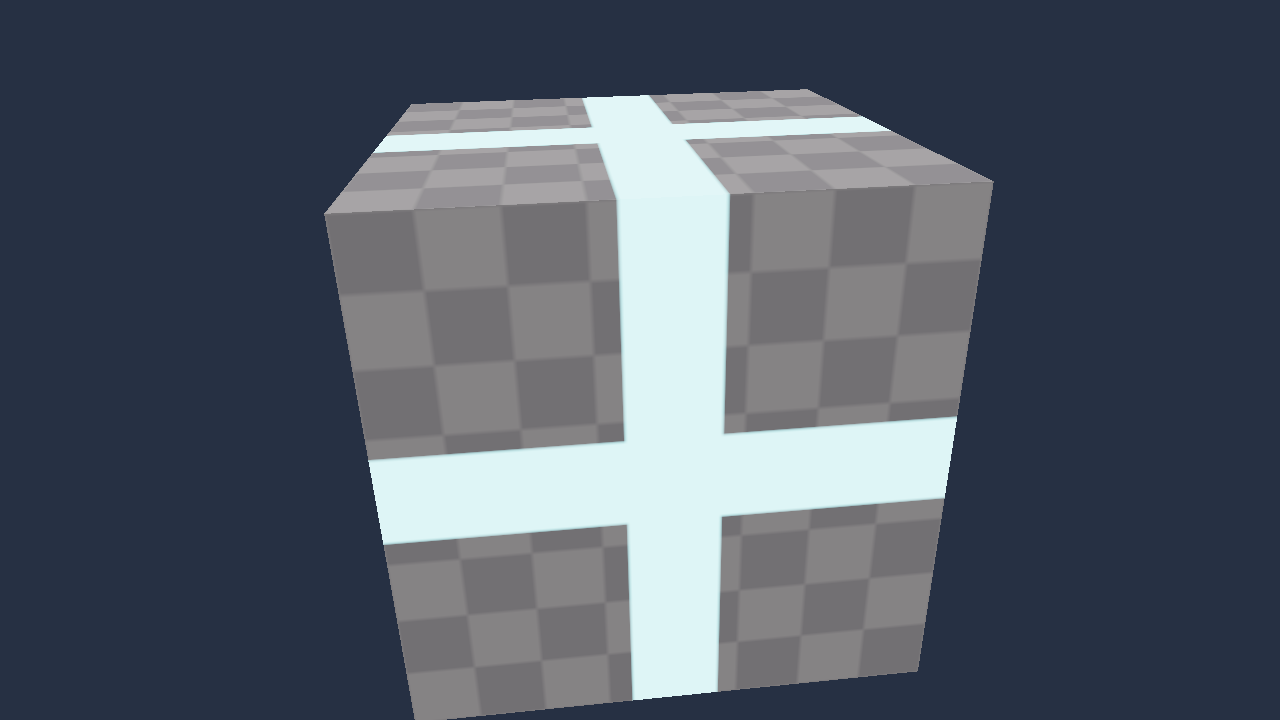
\includegraphics[width=\linewidth]{captura_bloom_desativado.png}
        \textbf{(a) Sem Bloom (LDR puro)}
    \end{minipage}
    \hfill
    \begin{minipage}{0.48\textwidth}
        \centering
        
\includegraphics[width=\linewidth]{captura_bloom_ativo.png}
        \textbf{(b) Com Bloom Ativo}
    \end{minipage}
    \caption{Comparação direta gerada pelo protótipo Vulkan. Em (a), a faixa incandescente sofre corte abrupto sem simulação de dispersão; em (b), o pipeline completo de 11 passes produz o espalhamento suave da luz (\textit{light bleeding}) ao redor do objeto, conferindo a percepção física de extrema luminância.}
    \label{fig:comparativo_bloom}
\end{figure}

\subsection{Interatividade e Usabilidade do Protótipo}
O protótipo permite intervenção direta do usuário em tempo de execução através das seguintes teclas:
\begin{itemize}
    \setlength{\itemsep}{0pt}
    \item \textbf{Barra de Espaço:} Alterna instantaneamente entre o modo com \textit{Bloom} ativo e o modo desativado, viabilizando a demonstração comparativa ao vivo.
    \item \textbf{Teclas \texttt{+} e \texttt{-}:} Aumentam e diminuem a intensidade do espalhamento luminoso ($\alpha$).
    \item \textbf{Tecla \texttt{ESC}:} Encerra a aplicação de forma limpa, garantindo a destruição ordenada de todos os semáforos, \textit{fences}, imagens e \textit{buffers} alocados na GPU.
\end{itemize}
\fussy
